На рисунке \ref{fig:CSA_Lookup_diff_texts} представлены сравнительные характеристики поиска
подстроки для различных текстовых данных.

\begin{figure}[h!]
    \centering
    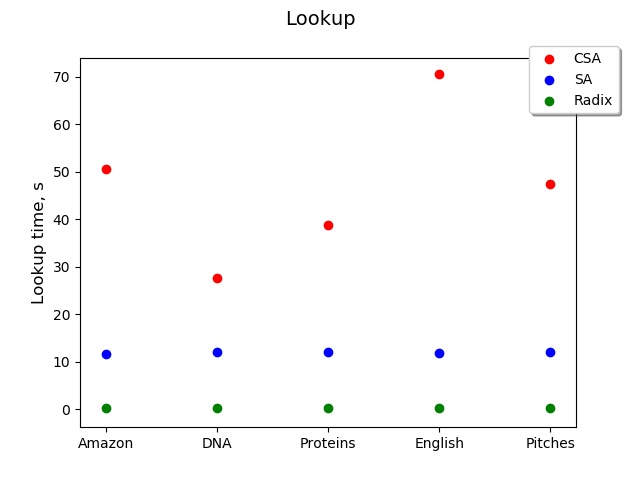
\includegraphics[width=12cm]{lookup_diff_texts}
    \caption{Поиск подстроки в CSA}
    \label{fig:CSA_Lookup_diff_texts}
\end{figure}

Рассмотрим относительное сжатие CSA по сравнению с suffix array. Рассчитывается среднее отношение памяти,
затраченной для работы CSA, к памяти, затраченной suffix array в зависимости от длины исходного текста.
На рисунке \ref{fig:CSA_compression_ratio_amazon} можно заметить уменьшение отношения, т.е. увеличение
коэффициента сжатия. Примечательно, что для малых размеров исходного текста CSA занимает больше места,
чем suffix array. Это объясняется наличием дополнительных структур данных, описанных на предыдущих страницах.
При построении CSA они занимают место, сопоставимое по порядку с размером индекса в сжатом виде.
Для больших текстов CSA становится более эффективным по сравнению с классическим suffix array.

\begin{figure}[h!]
    \centering
    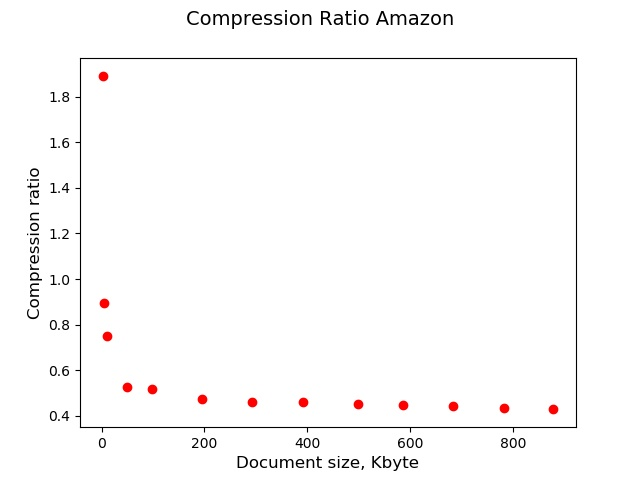
\includegraphics[width=12cm]{compression_ratio_amazon}
    \caption{Сжатие CSA по сравнению с SA}
    \label{fig:CSA_compression_ratio_amazon}
\end{figure}

\clearpage
Относительное сжатие CSA/SA для различных текстов показано на рисунке \ref{fig:CSA_compression_ratio_dif_texts}.
Можно явным образом заметить зависимость размера сжатого индекса от мощности алфавита, чего нельзя
сказать о suffix array и radix tree.

\begin{figure}[h!]
    \centering
    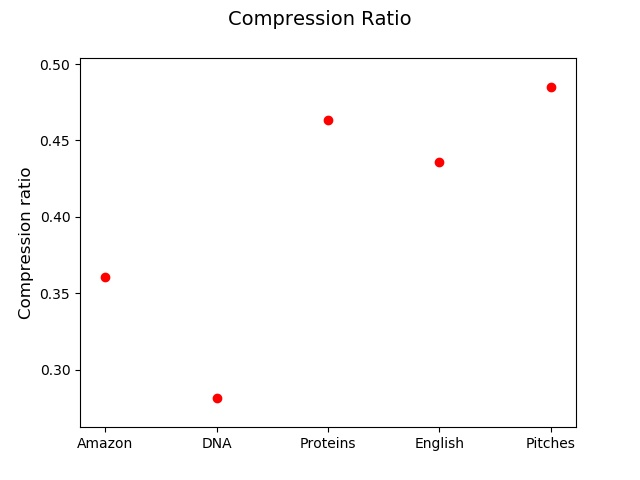
\includegraphics[width=12cm]{compression_ratio_dif_texts}
    \caption{Сжатие CSA по сравнению с SA}
    \label{fig:CSA_compression_ratio_dif_texts}
\end{figure}